\section{Kết quả thực nghiệm}
\subsection{Chất lượng truy xuất trên ba bộ}
\begin{table}[H]
\centering\small
\caption{Recall@5 và số câu tìm đủ mọi gold, sau sửa lỗi}
\begin{tabular}{llrrr}
\toprule Bộ & Phương pháp & Có gold & Recall@5 & All-gold\\
\midrule
30 câu & RAG vector & 25 & 0,7400 & 17/25\\
 & Hybrid & 25 & 0,7200 & 15/25\\
 & GraphRAG & 25 & 0,7800 & 16/25\\
\midrule
8 quan hệ & RAG vector & 8 & 0,2500 & 1/8\\
 & Hybrid & 8 & 0,6250 & 5/8\\
 & GraphRAG & 8 & 1,0000 & 8/8\\
\midrule
20 câu & RAG vector & 16 & 0,6250 & 8/16\\
 & Hybrid & 16 & 0,5938 & 8/16\\
 & GraphRAG & 16 & 0,7813 & 11/16\\
\bottomrule
\end{tabular}
\end{table}
\sourcefile{evaluation/runs/research_20261001/retrieval_summary.csv}

\begin{figure}[H]
\centering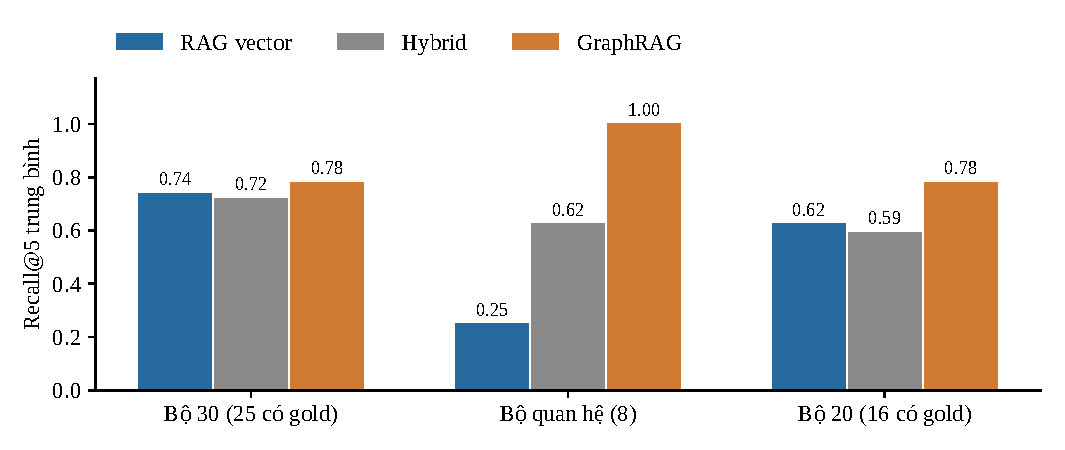
\includegraphics[width=\textwidth]{figures/recall_suites.pdf}
\caption{So sánh truy xuất; ba bộ có chồng lấp, không cộng thành mẫu độc lập.}
\end{figure}

Trên bộ 30, mức tăng Recall của GraphRAG so với RAG là 0,04, nhưng All-gold giảm một câu. Kết quả này cho thấy việc chọn một chỉ số duy nhất có thể dẫn đến kết luận thiếu cân bằng. Trên bộ quan hệ, hybrid đã tăng Recall 0,375 so với vector thuần; phần tăng thêm từ hybrid tới GraphRAG cũng là 0,375. Tín hiệu từ vựng vì vậy có đóng góp quan sát được trước khi xét đồ thị.

Trên bộ 20 có phạm vi rõ, GraphRAG tìm đủ gold ở 11/16 câu, hai đối chứng đạt 8/16. Chênh lệch với bộ 30 không thể được coi là tác động riêng của sửa code: phân bố nhóm và câu chữ đều khác. Bộ quan hệ có lợi thế thiết kế cho các cạnh đã xây; Recall bằng 1 ở đây là kết quả trên tám câu nội bộ, chưa là ước lượng cho mọi câu hỏi quan hệ mới.

\subsection{Phân nhóm và chất lượng đáp án}
\begin{figure}[H]
\centering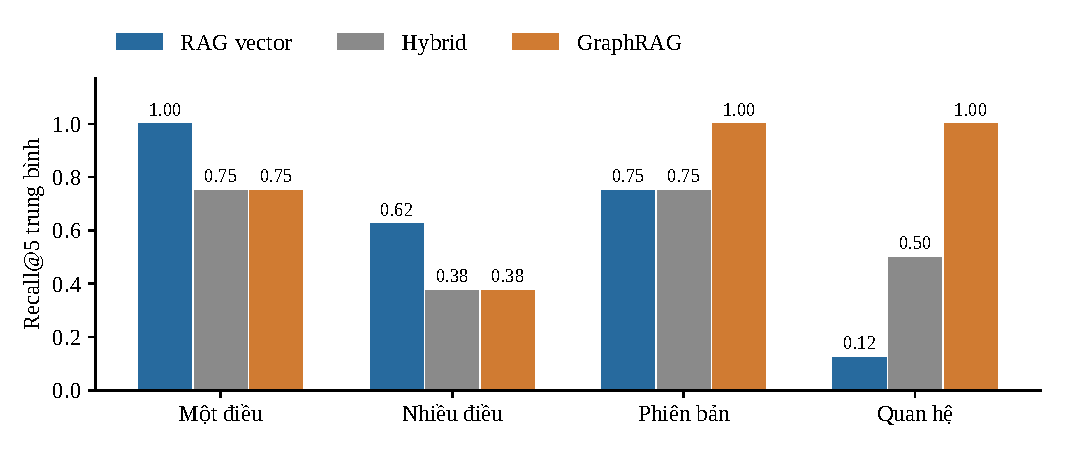
\includegraphics[width=\textwidth]{figures/recall_groups.pdf}
\caption{Recall@5 của bộ 20: mỗi nhóm trong hình có bốn câu có gold.}
\end{figure}

Nhóm một điều: RAG đạt 1,00, hybrid và GraphRAG cùng 0,75. Nhóm nhiều điều: RAG 0,625, hai phương pháp còn lại 0,375. Nhóm phiên bản: GraphRAG 1,00, hai đối chứng 0,75. Nhóm quan hệ: RAG 0,125, hybrid 0,50, GraphRAG 1,00. Đồ thị không tự bảo đảm cải thiện khi nhiều điều kiện nằm trong một văn bản; cạnh tranh top 5 và chọn phạm vi vẫn có thể làm mất chứng cứ.

\begin{table}[H]
\centering\small
\caption{Đánh giá nội dung sơ bộ bằng trợ lý AI, chưa chấm người độc lập}
\begin{tabular}{lcc}
\toprule Chỉ số & RAG vector & GraphRAG\\
\midrule
Đúng ý chính/phạm vi & 8/16 (50,00\%) & 11/16 (68,75\%)\\
Đủ ý theo gold & 4/16 (25,00\%) & 8/16 (50,00\%)\\
Nguồn hỗ trợ phát biểu & 9/16 (56,25\%) & 12/16 (75,00\%)\\
Từ chối phù hợp ngoài corpus & 4/4 & 4/4\\
\bottomrule
\end{tabular}
\end{table}
\sourcefile{evaluation/runs/research_20261001/answer_scores.json}

\begin{table}[H]
\centering\small
\caption{Số câu đạt đúng/đủ/nguồn trong từng nhóm, mẫu số mỗi ô là 4}
\begin{tabular}{lcc}
\toprule Nhóm & RAG & GraphRAG\\
\midrule
Một điều & 4 / 2 / 4 & 3 / 1 / 3\\
Nhiều điều & 1 / 0 / 2 & 0 / 0 / 1\\
Phiên bản & 3 / 2 / 3 & 4 / 3 / 4\\
Quan hệ & 0 / 0 / 0 & 4 / 4 / 4\\
\bottomrule
\end{tabular}
\end{table}

Mức tăng 3 câu đúng của GraphRAG tương ứng 18,75 điểm phần trăm trên 16 câu. Có 5 cặp GraphRAG thắng, 2 cặp RAG thắng và 9 cặp bằng nhau. Lợi ích tập trung ở 4 câu quan hệ và V02; bất lợi nằm ở S07 và M01. Với $p=0{,}4531$, chưa đủ bằng chứng ở mức 0,05 về ưu thế chung. Cả hai xử lý phù hợp bốn câu ngoài corpus, nhưng mẫu này chưa bao gồm toàn bộ kiểu yêu cầu thiếu chứng cứ.

\subsection{Độ trễ và lượng token}
\begin{table}[H]
\centering\small
\caption{Chi phí quan sát trên 20 lượt sinh của mỗi phương pháp}
\begin{tabular}{lrr}
\toprule Chỉ số & RAG vector & GraphRAG\\
\midrule
Độ trễ trung bình pipeline (ms) & 1.636,32 & 1.747,54\\
Độ trễ trung vị pipeline (ms) & 1.486,55 & 1.709,29\\
Token vào tổng & 29.484 & 31.723\\
Token ra tổng & 1.735 & 2.549\\
Token tổng & 31.219 & 34.272\\
\bottomrule
\end{tabular}
\end{table}
\sourcefile{evaluation/runs/research_20261001/generation_revalidated.json}

\begin{figure}[H]
\centering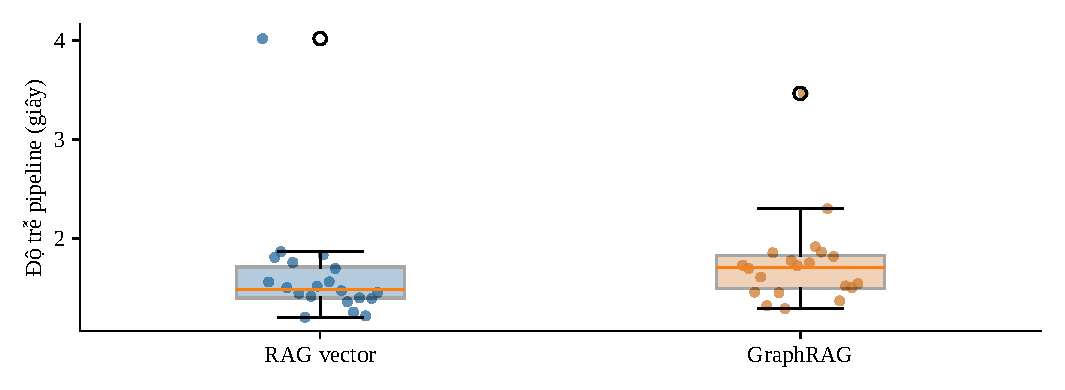
\includegraphics[width=\textwidth]{figures/latency.pdf}
\caption{Phân bố 20 độ trễ mỗi phương pháp; loại thời gian chờ pacing.}
\end{figure}

GraphRAG tăng khoảng 111,22 ms trung bình, tương đương 6,8\% so với RAG trong run này. Tổng token tăng 3.053, khoảng 9,8\%; token đầu ra tăng vì có thêm câu trả lời và nội dung dài hơn. RAG từ chối sai 7/16 câu có đáp án, GraphRAG từ chối sai 3/16. Vì thế, token thấp hơn của RAG một phần gắn với việc không trả lời câu có thể trả lời; chưa thể coi đó là ưu thế hiệu quả độc lập với chất lượng.

Độ trễ truy xuất trung vị trên bộ 30 lần lượt là 9,705 ms, 11,895 ms và 13,480 ms cho RAG, hybrid và GraphRAG. Trung bình tương ứng là 49,872 ms, 31,522 ms và 14,127 ms. Sự đảo thứ tự giữa trung bình và trung vị thể hiện ảnh hưởng của outlier trong điều kiện có tiến trình khác hoạt động. Không sử dụng các trung bình này để khẳng định GraphRAG luôn nhanh hơn truy xuất vector.

Khoảng cách nhỏ nhất giữa thời điểm bắt đầu 40 request là 5,000067 giây, phù hợp nhịp đã cấu hình. Chờ pacing và thời gian nạp model không nằm trong độ trễ bảng. Người dùng thực tế có thể chờ lâu hơn độ trễ pipeline nếu phải xếp hàng. Nghiên cứu không quy đổi token sang tiền, không đo thông lượng tải lớn và không suy ra thời gian phục vụ nhiều người dùng từ số đo đơn lẻ.
